% TeX encoding = utf8
% TeX spellcheck = pl_PL 
\documentclass[a4paper, 11pt]{article}
\usepackage[utf8]{inputenc}
\usepackage[polish]{babel}
\usepackage{polski}
\usepackage{float}
\usepackage{graphicx}
\usepackage{listings}
\usepackage{amsfonts}
\usepackage{geometry}
\usepackage{multicol}
\usepackage{latexsym}
\usepackage{enumerate}
\usepackage{hyperref}
\usepackage{wrapfig}
\usepackage{color} %red, green, blue, yellow, cyan, magenta, black, white
\definecolor{mygreen}{RGB}{28,172,0} % color values Red, Green, Blue
\definecolor{mylilas}{RGB}{170,55,241}

\author{Kamil Foryszewski}
\title{Sterowanie Procesami - projekt 2, zadanie 2.16}
\frenchspacing

\newgeometry{tmargin=2cm, bmargin=2cm, lmargin=2cm, rmargin=2cm}
\pagestyle{empty}


\begin{document}

\lstset{language=Matlab,%
    basicstyle=\color{red},
    breaklines=true,%
    morekeywords={matlab2tikz},
    keywordstyle=\color{blue},%
    morekeywords=[2]{1}, keywordstyle=[2]{\color{black}},
    identifierstyle=\color{black},%
    stringstyle=\color{mylilas},%
    commentstyle=\color{mygreen},%
    showstringspaces=false,
    numbers=right,%
    numberstyle={ \color{black}},% size of the numbers
    numbersep=5pt, % this defines how far the numbers are from the text
    emph=[1]{for,endfor,endwhile,endfunction,endif,break},emphstyle=[1]\color{blue}, %some words to emphasise
    emph=[2]{,.}, emphstyle=[2]\color{yellow},%
}

\maketitle
\tableofcontents

\section{Polecenie}
Obiekt regulacji jest opisany transmitancją: 
$$G(s) = \frac{K_0e^{-T_0s}}{(T_1 + 1)(T_2+1)}  = \frac{5e^{-T_0s}}{10.04s^2+7.02s +1}  $$
Gdzie: 
$K_0 = 3.5, T_0 = 5, T_1 = 2, T_2 = 5.02$

\section{Transmitancja dyskretna}
Wyznaczona transmitancja dyskretna ma następującą postać: 
$$G(z) = z^{-10}\frac{0.0388z+0.0346}{z^2-1.684z+0.705}$$
Została wyznaczona przy pomocy polecenia \emph{c2d} pakietu matlab. 
\begin{figure}[htp]
\centering
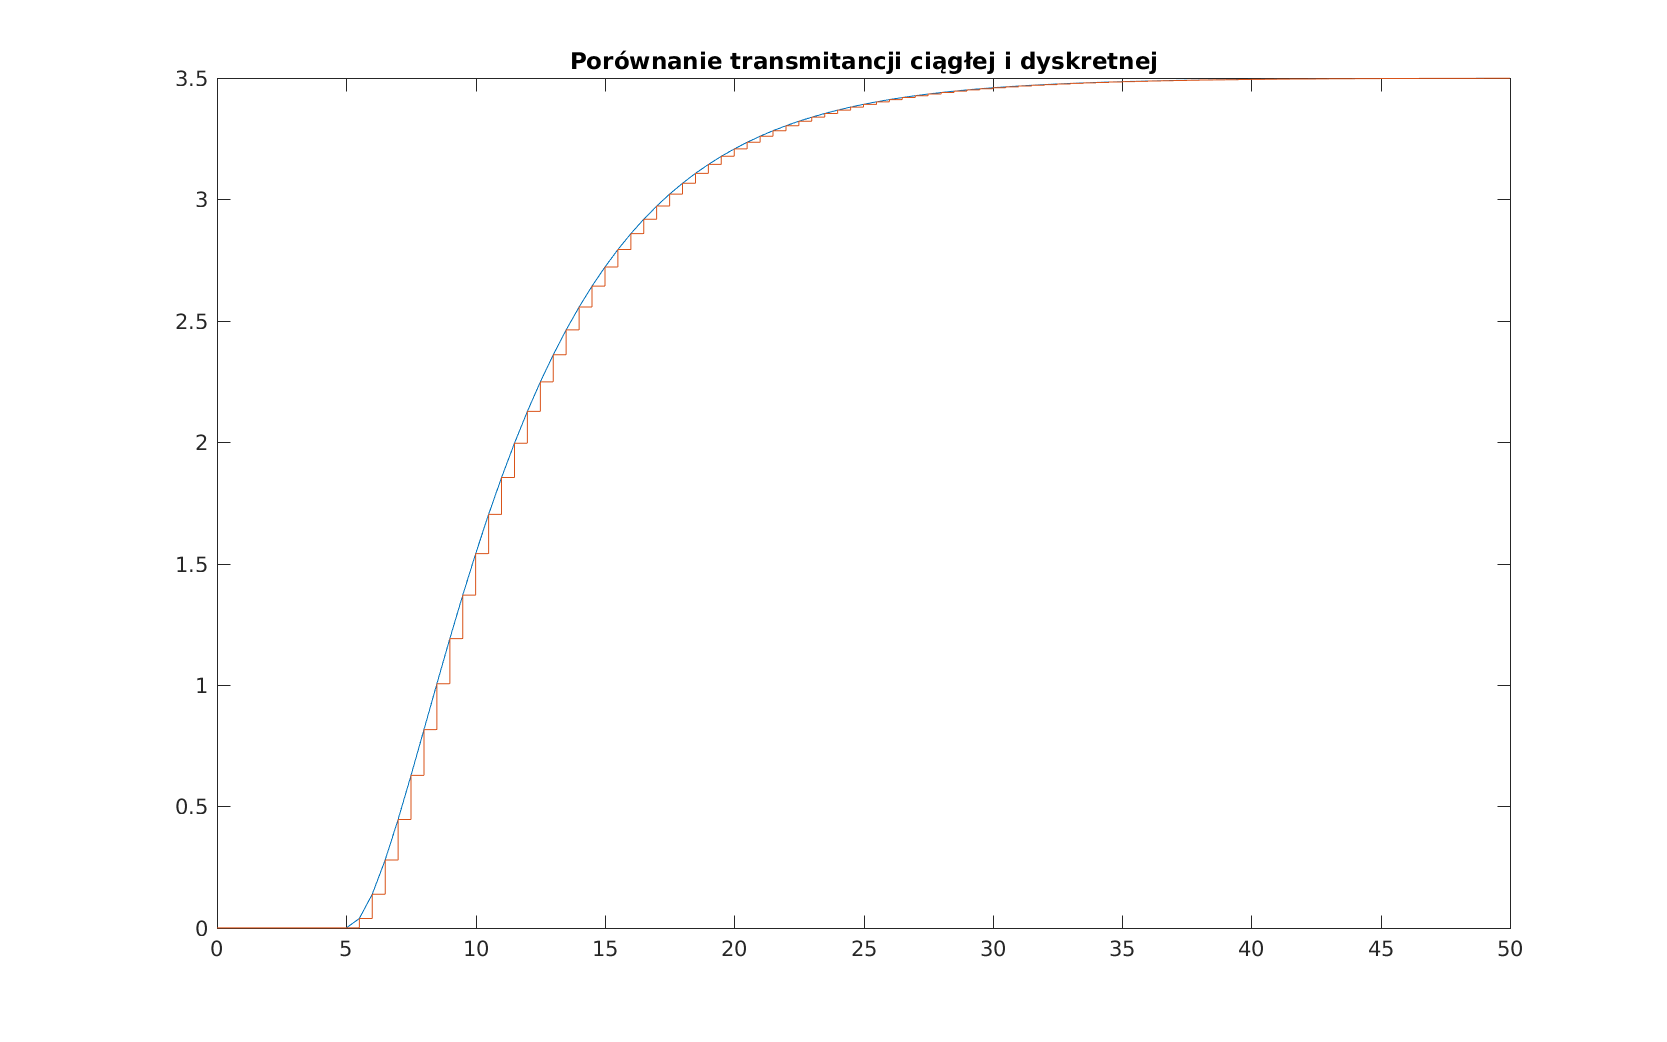
\includegraphics[scale=0.6]{1_1.png}
\caption{Odpowiedź skokowatransmitancji ciągłej i dyskretnej}
\label{}
\end{figure}%tutaj rysuneczek z matlaba 
Odpowiedź skokowa obu transmitancji w przybliżeniu jest taka sama. Odpowiedzi skokowe obliczone jako granice transmitancji przy argumentach $s$dążącym do $0$ i $z$ dażącym do $1$ są również bardzo zbliżone. Wzmocnienie statyczne transmitancji ciągłej $K_c = 5$, natomiast wzmocnienie statyczne transmitancji dyskretnej $K_d = 5.0572$
\section{Równanie różnicowe}
Korzystając z transmitancji możemy wyznaczyć równanie różnicowe opisujące obiekt w postaci: 

$$y(k) = \sum_{i=1}^{n} b_iy(k-i)+ \sum_{i=1}^{m} c_iu(k-1)$$
Należy zatem przekształcić transmitancję do następującej postaci: 
$$G(z) = \frac{0.0388z^{-11}+0.0346z^{-12}}{z-1.684z^{-1}+0.705z^{-2}} = \frac{Y(z)}{U(z)}$$
Po przekształceniu: 
$$Y(z)(1-1.6840z^{-1}+0.7050z^{-2}) = U(z)(0..388z^{-11}+0.0346z^{-12})$$
Skąd możemy bezpośrednio przejść do równania różnicowego: 
$$y(k) = 1.684(k-1) - 0.705(k-2) + 0.388u(k-11) + 0.0346u(k-12)$$


\section{Dobór regulatora PID metodą Zieglera-Nicholsa}




\end{document}